Sur base de l'étude de la communication audio, disponible dans le \href{https://gitlab.com/mosee/elech309-2024}{gitlab du projet}, cette partie du projet concerne la réalisation :

\begin{enumerate}
    \item[$\bullet$] d'un signal modulé en fréquence et suivant un format de trame donné
    \item[$\bullet$] d'une chaîne d'acquisition
    \item[$\bullet$] de la démodulation du signal
    \item[$\bullet$] de l'appel à la fonction qui exécute la commande\footnote{Cette fonction a été écrite précédemment, elle fait partie de la partie mécanique du projet. On doit juste passer en argument le signal démodulé}
\end{enumerate}

Nous n'avons pas besoin de réaliser le premier point puisque des exemples de signaux sont déjà disponibles sur l'UV. Par ailleurs, on peut remarquer que contrairement à ce qui est conseillé, on a décidé d'utiliser un seul dsPIC. Tout ceci est repris sur la Figure \ref{fig:bloc_com}

\begin{figure}[H]
    \centering
    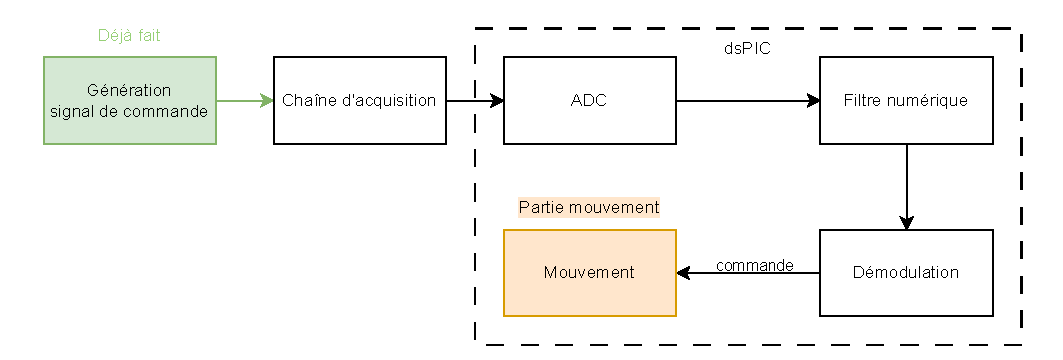
\includegraphics[scale=0.8]{pdffiles/diagramme_comm.pdf}
    \caption{Schéma-bloc de la partie communication}
    \label{fig:bloc_com}
\end{figure}